\documentclass[a4paper,11pt]{article}
\input{/home/tof/Documents/Cozy/latex-include/preambule_doc.tex}
\input{/home/tof/Documents/Cozy/latex-include/preambule_commun.tex}
\newcommand{\showprof}{show them}  % comment this line if you don't want to see todo environment
\setlength{\fboxrule}{0.8pt}
\fancyhead[L]{\fbox{\Large{\textbf{Lang 06}}}}
\fancyhead[C]{\textbf{Exercices fonctions}}
\newdate{madate}{10}{09}{2020}
%\fancyhead[R]{\displaydate{madate}} %\today
\fancyhead[R]{Première - NSI}
\fancyfoot[L]{\vspace{1mm}Christophe Viroulaud}
\AtEndDocument{\label{lastpage}}
\fancyfoot[C]{\textbf{Page \thepage/\pageref{lastpage}}}
\fancyfoot[R]{\includegraphics[width=2cm,align=t]{/home/tof/Documents/Cozy/latex-include/cc.png}}

\begin{document}
\begin{exo}
    Écrire la fonction \textbf{est\_pair(x: int) $\rightarrow$ bool} qui renvoie \textbf{\texttt{True}} si l'entier \textbf{\texttt{x}} est pair, \textbf{\texttt{False}} sinon.
\end{exo}
\begin{exo}
    Écrire la fonction \texttt{\textbf{valeur\_absolue(x: int) $\rightarrow$ int}} qui renvoie la valeur absolue de l'entier \textbf{\texttt{x}}.
\end{exo}
\begin{exo}
    Écrire la fonction \texttt{\textbf{surface(r: float) $\rightarrow$ float}} qui renvoie l'aire d'un cercle de rayon \textbf{\texttt{r}}. Le type \textbf{\texttt{float}} représente un nombre réel.
\end{exo}
\begin{exo}
    Écrire la fonction \texttt{\textbf{est\_majeur(age: int) $\rightarrow$ bool}} qui renvoie \textbf{\texttt{True}} si la personne d'âge \textbf{\texttt{age}} est majeure, \textbf{\texttt{False}} sinon.
\end{exo}
\begin{exo}
    Écrire la fonction \texttt{\textbf{puissance(x: int, n: int) $\rightarrow$ int}} qui renvoie \textbf{\texttt{x}} à la puissance \textbf{\texttt{n}}. Pour rappel $x^n = \underbrace{x×x×....×x}_{n}$. On utilisera une boucle pour effectuer le calcul.
\end{exo}
\begin{exo}
    Écrire la fonction \textbf{\texttt{lancer\_des() $\rightarrow$ int}} qui simule le lancer de deux dés à six faces et renvoie la somme des valeurs obtenues.
\end{exo}
\begin{exo}
    Écrire la fonction \texttt{\textbf{pythagore(a: int, b: int, c: int) $\rightarrow$ bool}} qui renvoie \textbf{\texttt{True}} si le triangle formé par les côtés de mesures \textbf{\texttt{a b c}} est rectangle. On supposera que les mesures sont des entiers donnés dans l'ordre croissant.
\end{exo}
\begin{exo}
    Écrire la fonction \textbf{\texttt{somme(n: int) $\rightarrow$ int}} qui renvoie la somme des entiers de 1 à n.
\end{exo}
\begin{exo}
    Écrire la fonction \textbf{\texttt{est\_premier(n: int) $\rightarrow$ bool}} qui renvoie \textbf{\texttt{True}} si \textbf{\texttt{n}} est premier.
\end{exo}
\begin{exo}
    Le calcul $0,5×(x+\frac{a}{x})$ permet d'effectuer une bonne approximation de $\sqrt{a}$ si on choisit une valeur de $x$ pas trop éloignée $\sqrt{a}$. Par exemple, pour $\sqrt{50}$ on choisit $x=7$.
    \begin{itemize}
        \item $0,5×(7+\frac{50}{7})\simeq 7,0714$
        \item $0,5×(7,0714+\frac{50}{7,0714})\simeq 7,0711$
        \item \dots
        \item après 20 itérations, on trouve: 7,0710678118654755
    \end{itemize}
    Et la calculatrice donne une valeur $\sqrt{50}=7,0710678118654755$
    \begin{enumerate}
        \item Écrire la fonction \textbf{\texttt{valeur\_proche(a: int) $\rightarrow$ int}} qui renvoie l'entier inférieur le plus proche de $\sqrt{a}$. Par exemple, l'appel \textbf{\texttt{valeur\_proche(50)}} doit renvoyer \textbf{\texttt{7}}. Pour trouver ce nombre il faut remarquer que $7^2 = 49 < 50$.
        \item Écrire la fonction \textbf{\texttt{racine(a: int) $\rightarrow$ float}} qui renvoie la racine carrée de \textbf{\texttt{a}}. La fonction utilisera la formule présentée en début d'exercice.
    \end{enumerate}
\end{exo}
\begin{exo}
    Turtle
    \begin{enumerate}
        \item Écrire une fonction \texttt{\textbf{triangle(c)}} qui trace un triangle de côté \textbf{\texttt{c}}.
        \item Écrire le programme qui affiche la figure \ref{sapin}.
              \begin{center}
                  \centering
                  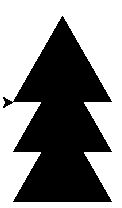
\includegraphics[width=2cm]{ressources/sapin.png}
                  \captionof{figure}{Sapin}
                  \label{sapin}
              \end{center}
    \end{enumerate}
\end{exo}
\end{document}